In this section we consider operations on unordered collections, namely: bags and sets.

\newpage\subsection{union(exp)}
The models for union between sets, and any other combination of bag and set, are very similar.
For both of these models, we simply append both arrays of variables, and apply the right type casting operation to ensure conformance.

Consider the expression \inlineocl{src.union(exp)}, where \inlineocl{src} is an expression resulting in a set of objects or integers, and \inelineocl(exp) is (an expression resulting in) a set of objects or an integers: the output of the operation is the set equal to the union of \inlineocl{src} and \inlineocl{exp}.
Reformulation using Global Constraints:
\begin{equation}\label{csp:union_setset}
    union\_setset(X,Y,Z):
    \begin{cases}
        X \;\mathbin{\|}\; Y'
        asSet(Y',Y)
    \end{cases}
\end{equation}

Consider the expression \inlineocl{src.union(exp)}, where \inlineocl{src} is an expression resulting in a set or bag of objects or integers, and \inelineocl(exp) is (an expression resulting in) a bag of objects or an integers: the output of the operation is the bag equal to the union of \inlineocl{src} and \inlineocl{exp}.
Reformulation using Global Constraints:
\begin{equation}\label{csp:union_Xbag}
    union\_Xbag(X,Y,Z):
    \begin{cases}
        X \;\mathbin{\|}\; Y'
        asBag(Y',Y)
    \end{cases}
\end{equation}

\newpage\subsection{Intersection}
Consider the expression \inlineocl{src.intersection(exp)}, where \inlineocl{src} is an expression resulting in a set or bag of objects or integers, and \inelineocl(exp) is (an expression resulting in) a set or bag of objects or integers: the output of the operation is the bag equal to the intersection of \inlineocl{src} and \inlineocl{exp}.
Reformulation using Global Constraints:
\begin{equation}\label{csp:intersection}
    intersection(X,Y,Z):
    \begin{cases}
        count(x_i,X,c_i)\\
        count(x_i,Y,c_i')\\
        count(x_i,Z,c_i'')\\
        c_i'' = \llbracket x_i = d \rrbracket * a_i + \llbracket x_i \neq d \rrbracket * min(c_i,c_i')\\
        a_i \geq max(c_i,c_i')\\
        count(z_i,X,b_i)\\
        count(z_i,Y,b_i')\\
        count(z_i,Z,b_i'')\\
        b_i'' = \llbracket z_i = d \rrbracket * a_i' + \llbracket z_i \neq d \rrbracket *min(b,b_i')\\
        a_i' \geq max(b_i,b_i')\\
    \end{cases}
\end{equation}
This model works for all combinations of set and bag, and will result in a set if either argument is a set.
This model can be divided in two similar parts: towards the output, and towards the input.
In the first part, towards the output, we count the occurrences of values of $X$, in $X$ and $Y$, and enforce the count of those values in $Z$ to be the minimum of the two.
In the second part, towards the input, we count the occurrences of values of $Z$, in $X$ and $Y$, and enforce the count of those values in $Z$ to be the minimum of the two.
This second part mainly ensures we don't slip in a value instead of a dummy.
We don't have a count for the exact number of dummies with this model, but we can enforce a lower bound: at least the greatest number of dummies in $X$ and $Y$.

\begin{figure}[!ht]
    \centering
    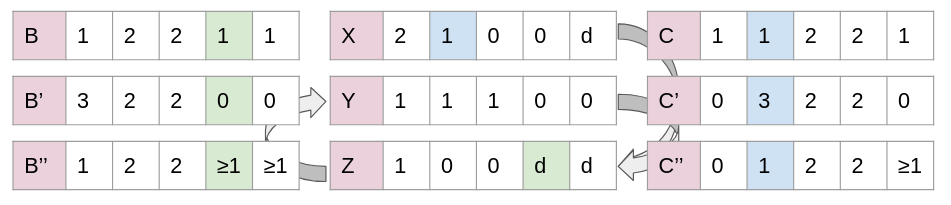
\includegraphics[trim={0 0 0 0},width=1\linewidth]{Contributions/OCLCSP/Operations/figures/intersectCount.png}
    \caption{Visualization of the use of count to model set and bag intersection}
    \label{fig:cumulative}
\end{figure}
In this figure we illustrate a solution and include all the intermediate variables.
In the middle we have $X$, $Y$, and $Z$.
On the right we have the \textit{towards the output} part,
and on the left, the \textit{towards the input} part.
Highlighted in blue we have $x_2$ and its counts in $X$, $Y$, and $Z$.
Highlighted in green we have the mirror with $z_4$ and its counts in $X$, $Y$, and $Z$.

% \begin{equation}\label{csp:intersection_setset}
%     intersection\_setset(X,Y,Z):
%     \begin{cases}
%         b_{i1} = x_i \wedge b_{i2} = 1\\
%         b_{(i+|X|)1} = y_i \wedge b_{i2} = 2\\
%         stable\_keysort(B,B',2)\\
%         c_n \iff (b_{n1}=b_{(n-1)1} \wedge b_{n2}\neq b_{(n-1)2})\\

%     \end{cases}
% \end{equation}

\newpage\subsection{unordered - unordered}
Consider the expression \inlineocl{exp1 - exp2}, where \inlineocl{exp1} is an expression resulting in a set or bag of objects or integers, and \inelineocl{exp2} is (an expression resulting in) a set or bag of objects or an integers: the output of the operation is the set or bag equal to the difference of \inlineocl{exp1} and \inlineocl{exp2}.
The type of the result is the same as \inlineocl{exp1}.
\begin{equation}\label{csp:diff_set}
    diff\_set(X,Y,Z):
    \begin{cases}
        count(x_i,Y,s_i)\\
        b_i \iff (s_i = 0)\\
        z'_i = d - (d-x_i)*\llbracket b_i \rrbracket\\
        sort(Z',\reverse{Z})
    \end{cases}
\end{equation}
This model can be seen as a filter on $X$ for values found in $Y$, and uses a similar model as that for \inlineocl{X.select(x | Y.count(x)=0)}.
And as the OCL describes, this model filters values from $X$ depending on their presence in $Y$, the result of which is in sorted into $Z$.


% \newpage
\subsection{symmetricDifference(exp)}
Consider the expression \inlineocl{src.symmetricDifference(exp)}, where \inlineocl{src} is an expression resulting in a set or bag of objects or integers, and \inelineocl{exp} is (an expression resulting in) a set or bag of objects or an integers: the output of the operation is the set or bag equal to the symmetric difference of \inlineocl{src} and \inlineocl{exp}.
The result of this operation is a set, if both arguments are sets.
\begin{equation}\label{csp:symdiff_set}
    symdiff\_set(X,Y,Z):
    \begin{cases}
        diff\_set(X,Y,S)\\
        diff\_set(Y,X,T)\\
        C = S \;\mathbin{\|}\; T\\
        sort(C,\reverse{Z})
    \end{cases}
\end{equation}
This model simply reuses the model for difference, filtering for both $X$ and $Y$.
The results, $S$ and $T$, are then combined and sorted into the output $Z$.

% \subsection{including}
% \begin{equation}\label{csp:setbagincluding}
%     including\_set(X,Y,Z):
%     \begin{cases}
%         diff\_set(X,Y,S)\\
%         diff\_set(Y,X,T)\\
%         C = S \;\mathbin{\|}\; T\\
%         sort(C,\reverse{Z})
%     \end{cases}
% \end{equation}


% \subsection{excluding}